\chapter{Data Processing}

Data Processing is the layer immediately following the Data Quality: once data have been formatted and cleansed, adapted then to our needs, we can start analysing and processing them through the use of adequate frameworks, in order to extract from, transform and enrich them for visualization purposes.\\

\section{Tecniche per il Data Processing}

\subsection{Batch Processing} \label{BatchProc}

\subsection{Graph Processing} \label{GraphProc}

\subsection{Stream Processing} \label{StreamProc}

Streaming data processing differentiates itself from the classic data processing for its use of unbounded datasets, that is a continuous and endless data flow which needs adequate abstractions in order to be able to apply operators or transformations like Map, Reduce and Filter operations. \\ 

Generally, there are 2 execution models usable when to approach an unbounded dataset:

\begin{itemize}
    \item \textbf{Streaming}: continuous elaboration as long as data are being produced.
    \item \textbf{(Micro-)Batch}: finite time execution, which releases resources when the batch processing ends.
\end{itemize}

A Batch based execution is feasible when requirements on the state management, in-order consuming and windowing are not present or very relaxed and, thus, a Streaming approach is generally favoured because of the conceptual paradigm which defines it: Dataflow Programming.

\paragraph{Dataflow Programming}  \label{DataflowProg}

Dataflow Programming is a programming paradigm which models an application as a Direct Acyclic Graph (DAG) and thus it differentiates itself very heavily from the Imperative Programming (or Control Flow), which models a program like finite sequence of operations.\\
This paradigm emphasizes the continuous flow of data between operators, defined as Black Boxes with explicit input and output ports used to connect with other operators. An operation runs as soon as all of its inputs become valid. Thus, dataflow languages are inherently parallel and can work well in large, decentralized systems \cite{Johnston:2004:ADP:1013208.1013209}.

\pagebreak
\section{Apache Spark} \label{Spark}

\pagebreak
\section{Apache Flink}\label{Flink}

\href{https://flink.apache.org/}{Apache Flink} is an open source framework developed for the continuous and distributed processing of data flows. Based on the Dataflow Programming model, it provides a set of abstractions specifically designed for real time stream processing.

\subsection{Abstraction levels}  \label{AbstractionLevels}

\begin{itemize}
	\item \textbf{Stateful Streaming}: It's the lowest abstraction layer, which allows developers to freely manage data flows and their processing, use fault-tolerant states and callback registration on events.
	\item \textbf{Core API}: it's the basic API, which is divided between \textbf{DataStream API}, specifically conceived for bounded and unbounded dataset processing, and \textbf{DataSet API}, implemented as a special case of the first API set, used only for bounded datasets. These 2 APIs offer transformations and operations like unions, aggregations, windowing and state management, needed for the data flow upon which they are applied.
	\item \textbf{Table API}: it's a declarative DSL \footnote{Domain Specific Language: a language with a limited expressiveness which focuses on a given domain of use.} which follows the extended relational model and offers the possibility to model a data stream like a table upon which it's possible to execute operations like projections, aggregations and groupings. Despite being less expressive with respect to the Core API, they allow for a greater compactness when it comes to describing the operations to be executed on the data.
	\item \textbf{SQL}: it's the highest level of abstraction offered by Flink and interacts directly with the Table APIs in order to provide a representation of the application being developed through SQL queries. It can be executed on the tables defined by the Table API, directly on the data.
\end{itemize}

\subsection{Programs Dataflows}  \label{ProgramsDataflows}

The base elements of a Flink application are the following:

\begin{itemize}
	\item \textbf{Streams}, data structures containing data.
	\item \textbf{Transformation Operators}, which can change the stream, for example, via aggregations, groupings, mappings and reductions.
	\item \textbf{Sources}, they are primary data entry points and can be files or records from queues like Kafka. They are the starting nodes of the application DAG.
    \item \textbf{Sinks}, They are the application output, being it a file, any process or another queue. They are the ending nodes of the application DAG.
\end{itemize}

\begin{code}

\begin{minted}[breaklines]{Scala}
val lines = env.addSource(new Consumer[String](...))

val events = lines.map(line -> parse(line))

val stats = events
            .keyBy("id") // Stream is partitioned by the key "id" 
            .timeWindow(Time.seconds(10)) // All the events in the given window are considered 
            .apply(MyWindowAggregationFunction()) // All the records are aggregated according to the function      

stats.addSink(new RollingSink(path))
\end{minted}

\end{code}

\begin{figure}[h]
	\centering
	\def\svgwidth{\columnwidth}
	\input{Figures/dataflow.pdf_tex}
	\decoRule
	\caption[Streaming Dataflow]{DAG outlining the previous code snippet}
	\label{fig:Dataflow}
\end{figure}

\paragraph{Windows}

\paragraph{Parallelism} \label{ParallelismFlink}

Applications using Flink are inherently parallels and distributed. During execution, a stream may be divided in more than one partition; each operator can have more than a single sub-task operating on data, each one independent from the other and executed on different threads or, if possible, on different machines or containers.\\
The parallelism of a task is the parameter indicating the number of subtasks an operator can have and, consequentially, the number of partitions of the stream getting outputted from that operator.\\

\begin{figure}[ht]
    \centering
    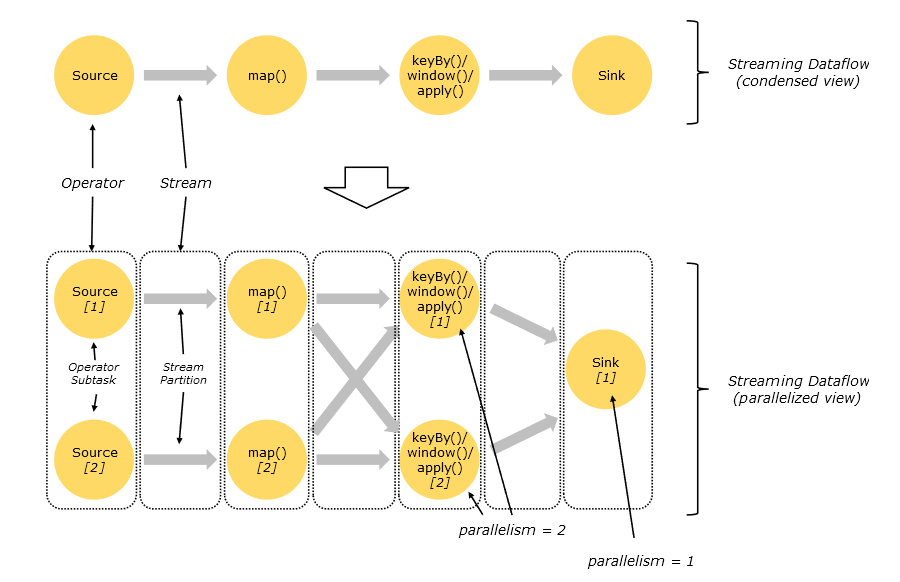
\includegraphics{Figures/parallel_dataflow.png}
    \decoRule
    \caption[Parallel Dataflow]{DAG with Parallelism=2}
    \label{fig:ParallelDataflow}
\end{figure}

Streams can transport data between a pair of operators following two different patterns: One-to-one pattern and redistributing pattern:
\begin{itemize}
	\item \textbf{One-to-one streams} preserve the stream partitioning and the order of the elements passed to the following operator. For example, the subtask[0] of a map() operator will get to see the same elements produced by the subtask[0] of the previous Source operator.
   
    \item \textbf{Redistributing streams} change their partitioning, sending the data to different subtasks, based on the transformation being applied. For example, a keyBy() operator repartitions the stream using the hash of the chosen key. In this case, the elements' order will be preserved only between neighbouring operations pairs, and won't be ever guaranteed being the same in the following operators.
\end{itemize}

\subsection{Data Streaming Fault Tolerance}

Flink offers built-in guarantees in case of failures, so that there's minimum disruption on the processing jobs and a consistent recovery of the data streaming applications' state. The two main features which allows recovery from errors or runtime exceptions are \textbf{Checkpoints} and \textbf{Savepoints}.

In case of a program failure (due to machine-, network-, or software failure), Flink stops the distributed streaming dataflow. The system then restarts the operators and resets them to the latest successful checkpoint. The input streams are reset to the point of the state snapshot. Any records that are processed as part of the restarted parallel dataflow are guaranteed to not have been part of the previously checkpointed state.

For this mechanism to realize its full guarantees, the data stream source (such as a message queue or a broker) needs to be able to rewind the stream to a defined recent point. Apache Kafka has this ability and Flink’s connector to Kafka exploits this ability.

\subsubsection{Checkpoints}

\begin{code}
    \label{code:checkpointing}
    \begin{minted}[breaklines, breakbefore=., breakafter=(]{Scala}
    val env: StreamExecutionEnvironment = StreamExecutionEnvironment.getExecutionEnvironment
    
    env.enableCheckpointing(60000)
    
    env.getCheckpointConfig.enableExternalizedCheckpoints(ExternalizedCheckpointCleanup.RETAIN_ON_CANCELLATION)
    
    env.setStateBackend(new FsStateBackend(state_dir, true)) 
    \end{minted}
    \captionof{listing}{An example of asynchronous checkpointing configuration on a FileSystem}
\end{code}~\\

\textbf{Checkpoints} are Flink's tool to guarantee automatic fault tolerance and recovery of the job's state, in case of runtime errors or failures. 
\\
\\
They are, essentially, snapshots of the current state of the job that act consistently as the system fall back in case of failure. Flink’s mechanism for drawing these snapshots is inspired by the standard Chandy-Lamport algorithm \cite{Chandy:1985:DSD:214451.214456} for distributed snapshots and is specifically tailored to Flink’s execution model \cite{DBLP:journals/corr/CarboneFEHT15}. 
\\
\\
Checkpointing must be configured on the application level as shown in the snippet \ref{code:checkpointing} by calling the \texttt{enableCheckpointing(milliseconds)} to specify how much time should pass between two consecutive snapshots. By default, if a job is cancelled the checkpoint is deleted as well, so the retainment on cancellation must be enabled manually. 
\\
\\
An additional configuration available to application level setup is the State Back-end, that is the location where the checkpoint, thus, the job's state, should be saved. There are three possible back-ends which can be chosen from: \textbf{in Memory}, useful for testing, on a \textbf{Filesystem} (local or distributed, like HDFS) and on \textbf{RocksDB}\footnote{\href{http://rocksdb.org/}{RocksDB} is an embeddable persistent key-value store for fast storage}, particularly recommended for huge states. Optionally, snapshots can be taken asynchronously in order not to block the processing pipeline.
Checkpoints can be used to manually recover from failures through specific commands from Flink CLI, but they don't support scaling on recovery, that is, parallelism can't be changed when recovering from a snapshot.

\paragraph{Barriers}

A core element in Flink’s distributed checkpointing are the \textit{stream barriers}. These barriers are injected into the data stream starting from the data source and flow with the records as part of the data stream, separating the records in the data stream belonging to two consecutive snapshots. Each barrier carries the ID of the snapshot whose records were pushed in front of it. Barriers do not interrupt the flow of the stream and are hence very lightweight. Multiple barriers from different snapshots can be in the stream at the same time, which means that various snapshots may happen concurrently.
\\
\begin{figure}[h]
    \centering
    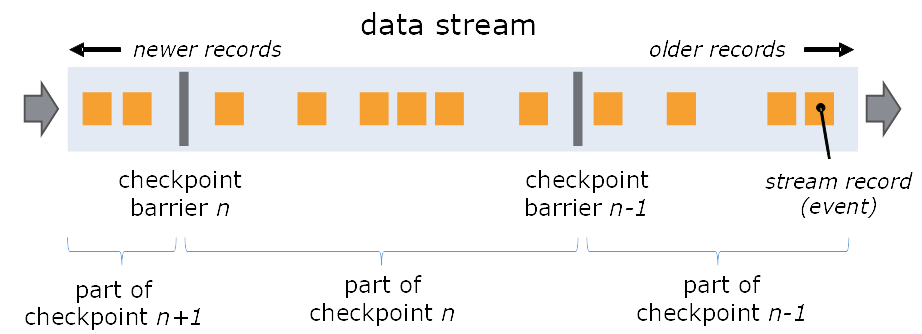
\includegraphics[width=0.7\linewidth]{Figures/stream_barriers}
    \caption{Visual representation of Stream Barriers}
    \label{fig:streambarriers}
\end{figure}
\\
The point where the barriers for snapshot $n$ are injected (let’s call it $S_n$) is the position in the source stream up to which the snapshot covers the data. For example, in \textbf{Apache Kafka}, this position would be the last record’s offset in the partition. This position $S_n$ is reported to the checkpoint coordinator, Flink’s JobManager.
\\
\\
The barriers then flow downstream: when an intermediate operator has received a barrier for snapshot $n$ from all of its input streams, it emits a barrier for snapshot $n$ into all of its outgoing streams. Once a sink operator (the end of a streaming DAG) has received the barrier $n$ from all of its input streams, it acknowledges that snapshot $n$ to the checkpoint coordinator. After all sinks have acknowledged a snapshot, it is considered completed.

Once snapshot $n$ has been completed, the job will never again ask the source for records from before $S_n$, since at that point these records (and their descendant records) will have passed through the entire data flow topology.
\\
\\
Operators that receive more than one input stream need to \textit{\textbf{align}} the input streams on the snapshot barriers:

\begin{itemize}
\item As soon as the operator receives snapshot barrier $n$ from an incoming stream, it cannot process any further records from that stream until it has received the barrier $n$ from the other inputs as well. Otherwise, it would mix records that belong to snapshot $n$ and with records that belong to snapshot $n+1$.
\item Streams that report barrier $n$ are temporarily set aside. Records that are received from these streams are not processed, but put into an input buffer.
\item Once the last stream has received barrier $n$, the operator emits all pending outgoing records, and then emits snapshot $n$ barriers itself.
\item After that, it resumes processing records from all input streams, processing records from the input buffers before processing the records from the streams.
\end{itemize}

\paragraph{Exactly Once vs. At Least Once}

The alignment step previously described may add latency to the streaming program. Usually, this extra latency is on the order of a few milliseconds, but some applications' latency may increase noticeably. If consistent super low latencies (few milliseconds) for all records is a strict requirement, Flink has a switch to skip the stream alignment during a checkpoint. Checkpoint snapshots are still drawn as soon as an operator has seen the checkpoint barrier from each input.

When the alignment is skipped, an operator keeps processing all inputs, even after some checkpoint barriers for checkpoint $n$ arrived. That way, the operator also processes elements that belong to checkpoint $n+1$ before the state snapshot for checkpoint $n$ was taken. On a restore, these records will occur as duplicates, because they are both included in the state snapshot of checkpoint $n$, and will be replayed as part of the data after checkpoint $n$.
\\
Alignment happens only for operators with multiple predecessors (join operators) as well as operators with multiple senders (such as a stream repartitioning/shuffle). Because of that, dataflows with only parallel streaming operations (\texttt{map()}, \texttt{flatMap()}, \texttt{filter()}, …) actually give \textit{exactly once} guarantees even in \textit{at least once} mode.

\subsubsection{Savepoints}

\begin{code}
    \label{code:savepoint}
    \begin{minted}{Bash}
flink savepoint <jobId> [<savepointDirectory>] -yid <yarnAppId> 
    \end{minted}
    \captionof{listing}{Savepoint triggering from the Flink CLI}
\end{code}~\\

\textbf{Savepoints}, just like checkpoints, serve the purpose to save the state of a Flink application in case of cancellation or failures. Differently from checkpoints, they can only be taken manually from Flink CLI, but support parallelism rescaling and they're the go-to choice when Flink's application computational capabilities must be improved by setting an higher parallelism factor or when an upgrade to a more recent version of Flink must be performed. Savepoint's mechanism works such that it associates each application's stateful operator, to its own state in a map-like structure: for this very reason, in order to successfully preserve state when upgrading a Flink application, each stateful operator needs to have its own \texttt{uid} set.

\subsection{High Availability}

A Flink's setup, being a standalone or a YARN cluster, is made of a Job Manager and one or more Task Managers, each one with one or more parallelism slots (cores usable for processing). Task Managers (TMs) handle jobs actual executions, while the Job Manager (JM) handles TM orchestration and monitoring and for this reason is a single point of failure. 

.......

\subsection{Flink Extensions} \label{FlinkLibs}

\subsubsection{FlinkCEP: Complex Events Processing}

FlinkCEP is a Flink extension adding the possibility to analyse events pattern in a DataStream, thanks to the Pattern API. This API allows the definition of patterns to be found in a stream and their selection in order to create a new DataStream of Alerts.\\


\begin{code}
\label{code:pattern-example}
\begin{minted}[breaklines]{Scala}

val input: DataStream[Event] = ...

val pattern = Pattern.begin("start").where(_.getId == 42)
.next("middle").subtype(classOf[SubEvent]).where(_.getVolume >= 10.0)
.followedBy("end").where(_.getName == "end")

val patternStream = CEP.pattern(input, pattern)

val result: DataStream[Alert] = patternStream.select(createAlert(_))
\end{minted}
\captionof{listing}{An example of Pattern API usage}
\end{code}~\\

In FlinkCEP, a \textbf{Pattern}, similarly to a pattern of a Regular Expression, can be \textbf{single} or \textbf{iterative}. For example, in a pattern like \texttt{"a b+ c? d"}, \texttt{a}, \texttt{c?} e \texttt{d} are single patterns, while \texttt{b+} is iterative.
\\

In a Pattern there can be, analogously to Regular Expressions, Quantifiers and Conditions.

\paragraph{Quantifiers}

Iterative patterns can be specified with the following self explanatory methods:

\begin{itemize}
    \item \texttt{pattern.oneOrMore()};
    \item \texttt{pattern.times(\#ofTimes)};
    \item \texttt{pattern.optional()}
\end{itemize}

\paragraph{Conditions}

Each pattern can have additional conditions specified, which can be related to a property of an incoming event, or the contiguity to other events.

Methods \texttt{pattern.where()} and \texttt{pattern.or()} can be used to specify \texttt{IterativeCondition}s, \texttt{SimpleCondition}s or a combination of multiple conditions. In this case, combinations can be specified concatenating all the previous methods, including the quantifiers, optionally adding more constraints on the contiguity of the same pattern by calling \texttt{consecutive()}, for the strict contiguity, and \texttt{allowCombinations()} for the relaxed non-deterministic contiguity.
\\
Some examples:

\begin{code}
\label{code:iterative-cond}
\begin{minted}[breaklines]{Scala}
middle.oneOrMore().where(
    (value, ctx) => {
        lazy val sum = ctx.getEventsForPattern("middle")
                          .asScala.map(_.getPrice).sum
        value.getName.startsWith("foo") && sum + value.getPrice < 5.0
    }
)
\end{minted}
\captionof{listing}{Iterative Condition}
\end{code}~\\

\begin{code}
    \label{code:simple-cond}
    \begin{minted}[breaklines]{Scala}
//Example of conjunction through where concatenation
start.where(event => event getName startsWith "foo" ) )
     .where(event => event getTotal equals 50  )

start.subtype(classOf[SubEvent]).where(subEvent => ... /* some condition */)
    \end{minted}
    \captionof{listing}{Conditions combinations}
\end{code}~\\

\paragraph{Pattern Combination}

Similarly to conditions combination, pattern combination is possible through the consecutive calls to the following methods allowing to specify the contiguity constraints which a given pattern should satisfy:

\begin{itemize}
    
    \item \texttt{next()}, for strict contiguity.
    \item \texttt{followedBy()}, for relaxed contiguity.
    \item \texttt{followedByAny()}, for non deterministic relaxed contiguity.
    \item \texttt{notNext()}, NOT pattern with strict contiguity.
    \item \texttt{notFollowedBy()}, NOT pattern with relaxed contiguity.

\end{itemize}

Each pattern combination can be followed by a time constraint specified by concatenating \texttt{within(Time)}.

\paragraph{Pattern Detection}

Once a pattern sequence has been specified, it needs to applied to the target \texttt{Datastream}, creating this way a \texttt{PatternStream}.
On this new stream \texttt{select} or \texttt{flatSelect} operations need to be applied in order to enable further processing on the events satisfying the pattern.

\subsubsection{Other extensions: Flink Gelly and FlinkML}

In addition to the aforementioned library for complex event handling, Flink makes specific sets of API available, which provide useful tools when it comes to enable advanced processing on data.

\paragraph{Flink Gelly} is an API based on the Flink \texttt{Dataset}s API specifically developed for Graph Processing. Graphs are stored as a finite set of vertices and edges, a special case of a \texttt{Dataset}. This library allows the application of operators like Map, Filter, Intersect and Union, Mutations like edge and vertex removal, but also advanced techniques belonging to Graph Theory like \textit{Iterative Graph Processing} (Vertex-centric, Scatter-Gather and Gather-Sum-Apply), \textit{Single Source Shortest Paths}, \textit{Clustering} and Similarity analysis.

\paragraph{FlinkML} is a set of tools which allows the application of Machine Learning techniques on Flink data streams, including both algorithmic implementations for supervised (\textit{SVMs} and \textit{Multiple Linear Regressors}) and unsupervised (\textit{K-nearest neighbours}) learning, Data Preprocessing and Recommendation (\textit{ALS}).


